% !TeX program = xelatex
\documentclass{article}
\usepackage{kotex}
\usepackage[a4paper, left=3cm, right=3cm, top=2.5cm, bottom=2.5cm]{geometry}
\usepackage{amsmath, amssymb}
\usepackage{tcolorbox}
\usepackage{caption}
\usepackage{setspace}
\usepackage{xcolor}
\usepackage{titlesec}
\usepackage{tikz}
\usetikzlibrary{arrows.meta, angles, quotes}

\setstretch{1.3}
\renewcommand{\figurename}{그림}
\titleformat{name=\section,numberless}
  {\normalfont\large\bfseries\color{blue}}{}
  {0pt}{}

\title{1.6 회전}
\date{}
\author{}

\begin{document}
\maketitle

\section*{1.6 회전}

\subsection*{평면에서의 회전}

\begin{tcolorbox}[
  colback=teal!4, colframe=teal!65!black,
  title=정의 \& 핵심 규칙,
  fonttitle=\bfseries, boxrule=0.5mm, arc=3mm]

\textbf{\textcolor{teal!65!black}{정의 (평면에서의 회전).}}\quad
$\mathbb{E}^2$에서의 회전은 주어진 \textbf{회전 중심} $C$ 주위로 각도 $\phi$만큼 평면을 돌리는 변환이다.
\begin{itemize}\setlength\itemsep{0pt}
  \item 반시계 방향 회전 $\to$ \textbf{양(+)의 각}
  \item 시계 방향 회전 $\to$ \textbf{음(-)의 각}
\end{itemize}
\textbf{표기.}\quad $R_{C,\phi} = \text{(중심 $C$, 각 $\phi$의 회전)}$

\noindent\textcolor{teal!50!black}{\rule{\linewidth}{0.4pt}}

\textbf{\textcolor{teal!65!black}{좌표 공식}} ($xy$평면, 원점 $O$ 중심):
\[
  R_{O,\phi}(x,\,y) \;=\; (x\cos\phi - y\sin\phi,\quad x\sin\phi + y\cos\phi)
\]
행렬 표현:
$R_{O,\phi} = \begin{pmatrix}\cos\phi & -\sin\phi \\ \sin\phi & \cos\phi\end{pmatrix}$

\noindent\textcolor{teal!50!black}{\rule{\linewidth}{0.4pt}}

\textbf{\textcolor{teal!65!black}{핵심 규칙 (역함수·합성).}}
\begin{itemize}\setlength\itemsep{2pt}
  \item \textbf{역함수}: $(R_{P,\phi})^{-1} = R_{P,-\phi}$
  \item \textbf{합성} (같은 중심): $R_{P,\phi_1} \circ R_{P,\phi_2} = R_{P,\,\phi_1+\phi_2}$
\end{itemize}

\end{tcolorbox}

\textbf{확인 (좌표 공식의 유도 --- 극좌표 이용).}\quad
$(x, y)$를 극좌표 $(r, \theta)$로 나타내면: $x = r\cos\theta,\; y = r\sin\theta$.
원점 $O$를 중심으로 각 $\phi$만큼 회전하면 극좌표에서 $\theta \mapsto \theta + \phi$이므로
\begin{align*}
  R_{O,\phi}(x,y)
    &= \bigl(r\cos(\theta+\phi),\; r\sin(\theta+\phi)\bigr) \\
    &= \bigl(r(\cos\theta\cos\phi - \sin\theta\sin\phi),\;
              r(\cos\theta\sin\phi + \sin\theta\cos\phi)\bigr) \\
    &= (x\cos\phi - y\sin\phi,\quad x\sin\phi + y\cos\phi)
\end{align*}
세 번째 등호에서 삼각함수 덧셈 공식과 $x=r\cos\theta$, $y=r\sin\theta$를 대입하였다.
\hfill $\square$

\begin{figure}[h]
\centering
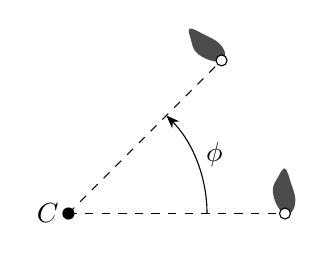
\begin{tikzpicture}[>=Stealth, scale=1.1]
  % Center C
  \fill (0,0) circle (2pt) node[left]{$C$};

  % Radius lines (dashed)
  \draw[dashed] (0,0) -- (2.5,0);          % to original position
  \draw[dashed] (0,0) -- (1.77,1.77);      % to rotated position (phi≈45°)

  % Arc showing angle phi
  \draw[->] (1.6,0) arc (0:45:1.6) node[midway, right, yshift=2pt]{$\phi$};

  % Original object (small blob at right)
  \begin{scope}[xshift=2.5cm]
    \draw[fill=black!70, draw=none]
      plot[smooth cycle, tension=0.65] coordinates {
        (0.00, 0.52)(-0.08, 0.42)(-0.14, 0.28)(-0.10, 0.11)
        (-0.01, 0.00)(0.08, 0.02)(0.12, 0.16)(0.07, 0.35)
      };
    \draw[fill=white] (0,0) circle (1.8pt);  % open circle at foot
  \end{scope}

  % Rotated object (same shape, rotated 45°)
  \begin{scope}[rotate=45, xshift=2.5cm]
    \draw[fill=black!70, draw=none]
      plot[smooth cycle, tension=0.65] coordinates {
        (0.00, 0.52)(-0.08, 0.42)(-0.14, 0.28)(-0.10, 0.11)
        (-0.01, 0.00)(0.08, 0.02)(0.12, 0.16)(0.07, 0.35)
      };
    \draw[fill=white] (0,0) circle (1.8pt);  % open circle at foot
  \end{scope}
\end{tikzpicture}
\caption{중심 $C$, 각 $\phi$의 회전 $R_{C,\phi}$}
\label{fig:1.14}
\end{figure}

\subsection*{공간에서의 회전}

\begin{tcolorbox}[
  colback=teal!4, colframe=teal!65!black,
  title=정의 (공간에서의 회전),
  fonttitle=\bfseries, boxrule=0.5mm, arc=3mm]

삼차원 공간에서의 회전 $R_{A,\phi}$는 \textbf{축} $A$(유향 직선)와 \textbf{각} $\phi$에 의해 결정된다.
\begin{itemize}\setlength\itemsep{0pt}
  \item 양의 회전 방향: \textbf{오른손 법칙} --- 엄지가 축의 방향을 가리키면 나머지 손가락이 굽는 방향
  \item 예: $z$축을 중심, 양의 방향($z$축 방향 양) $\Rightarrow$ $x$축 양의 방향에서 $y$축 양의 방향으로 $\phi$만큼 회전
\end{itemize}

\end{tcolorbox}

\begin{tcolorbox}[
  colback=red!4, colframe=red!60!black,
  title=정리: 평행 이동과 회전은 향(Orientation)을 보존,
  fonttitle=\bfseries, boxrule=0.5mm, arc=3mm]

평행 이동과 회전은 모두 \textbf{두 반사의 합성}으로 표현되며, 향을 보존한다.

\end{tcolorbox}

\textbf{증명.}\quad
먼저 평행 이동과 회전이 각각 두 반사의 합성으로 표현됨을 확인한다.
평행 이동의 경우 정리 1.5.1에 의해, 회전의 경우 문제 1.6.1에 의해 각각 두 반사의 합성으로 쓸 수 있다.

이제 각각의 반사는 향을 뒤바꾸지만,
향이 두 번 바뀌면 서로 상쇄되어 결국에는 처음 향으로 돌아온다.
즉 향이 보존된다.
\hfill $\square$

\subsection*{연습문제 1.6}

\begin{enumerate}
  \item \textbf{(문제 1.6.1)}\quad $\mathbb{E}^2$에서 두 직선 $L_1, L_2$가 점 $P$에서 만난다 하자.
    $f_1$은 $L_1$에 대한 반사, $f_2$는 $L_2$에 대한 반사라 할 때, 합성 $f_2 \circ f_1$은
    $P$를 중심으로 하는 회전이고 회전각은 $L_1$에서 $L_2$까지 잰 각의 두 배임을 보여라.\\
    \textit{(도움말: 정리 1.5.1의 증명을 모방하여라.)}

  \item \textbf{(문제 1.6.2)}\quad 임의의 점 $(a,b) \in \mathbb{R}^2$를 중심으로 각 $\phi$만큼의
    회전에 대한 공식을 구하여라.
\end{enumerate}

\end{document}
